\documentclass{sig-alternate-2013}

\newcommand{\mypar}[1]{\vspace{0.05in} \noindent \textbf{#1 \,}}

\usepackage[subscriptcorrection,slantedGreek,nofontinfo,lite]{mtpro2}
\usepackage[T1]{fontenc}

\usepackage{times}
\renewcommand{\rmdefault}{ptm}

\usepackage{color}
\usepackage{algorithmicx}
\usepackage[ruled]{algorithm}
\usepackage[noend]{algpseudocode}
\usepackage[final,expansion=alltext]{microtype}
\usepackage[english]{babel}

%\usepackage{natbib}
\usepackage[colorlinks,citecolor=blue, linkcolor=blue]{hyperref}

\usepackage[all]{hypcap}

\newcommand{\pluseq}{\mathrel{+}=}
\newcommand{\minuseq}{\mathrel{-}=}
\newcommand{\E}{\mathrm{E}}
\newcommand{\g}{\, | \,}

\newfont{\mycrnotice}{ptmr8t at 7pt}
\newfont{\myconfname}{ptmri8t at 7pt}
\let\crnotice\mycrnotice%
\let\confname\myconfname%

\permission{
Permission to make digital or hard copies of all or part of this work for personal or classroom use is granted without fee provided that copies are not made or distributed for profit or commercial advantage and that copies bear this notice and the full citation on the first page. Copyrights for components of this work owned by others than the author(s) must be honored. Abstracting with credit is permitted. To copy otherwise, or republish, to post on servers or to redistribute to lists, requires prior specific permission and/or a fee. Request permissions from Permissions@acm.org.}
\conferenceinfo{RecSys'15,}{September 16--20, 2015, Vienna, Austria. \\ 
{\mycrnotice{Copyright held by the authors. Publication rights licensed to ACM.  This is the authors' version of the work. It is provided for personal use, not for redistribution.}}}
\copyrightetc{ACM \the\acmcopyr}
\crdata{978-1-4503-3692-5/15/09\ ...\$15.00.
%DOI: http://dx.doi.org/10.1145/2792838.2800193}
}

\clubpenalty=10000
\widowpenalty = 10000

%format urls
\renewcommand\UrlFont{\color{blue}\rmfamily}


\begin{document}

\title{A Probabilistic Model for Using Social Networks in Personalized
  Item Recommendation}

\numberofauthors{3}
\author{
\alignauthor
Allison J.B. Chaney\\
       \affaddr{Princeton University}\\
       \email{achaney@cs.princeton.edu}
\alignauthor
David M. Blei\\
       \affaddr{Columbia University}\\
       \email{blei@cs.columbia.edu}
\alignauthor
Tina Eliassi-Rad\\
       \affaddr{Rutgers University}\\
       \email{eliassi@cs.rutgers.edu}
}


\maketitle
\begin{abstract}
Preference-based recommendation systems have transformed how we
consume media.  By analyzing usage data, these methods uncover our
latent preferences for items (such as articles or movies) and form
recommendations based on the behavior of others with similar tastes.
But traditional preference-based recommendations do not account for
the social aspect of consumption, where a trusted friend might point
us to an interesting item that does not match our typical preferences.
In this work, we aim to bridge the gap between preference- and
social-based recommendations.  We develop \textit{social
Poisson factorization} (SPF), a probabilistic model that incorporates social
network information into a traditional factorization method; SPF
introduces the social aspect to algorithmic
recommendation.  We develop a scalable algorithm for analyzing data
with SPF, and demonstrate that it outperforms competing methods
on six real-world datasets; data sources include a social reader and Etsy.
\end{abstract}

% A category with the (minimum) three required fields
%\category{H.3.3}{Information Search and Retrieval}{Information Filtering}
%A category including the fourth, optional field follows...

\keywords{Recommender systems; probabilistic models; social networks.}

\section{Introduction}
Recommendation has become a core component in our online
experience, such as when we watch movies, read articles, listen to
music, and shop.  Given information about what a user has consumed
(e.g., items viewed, marked as ``favorites,'' or rated), the goal of
recommendation is to suggest a set of unobserved items that she will
like.

\addtocounter{footnote}{-1}
\begin{figure}[t]
\centering
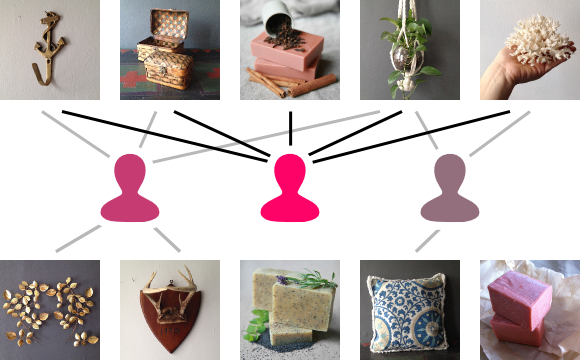
\includegraphics[width=\columnwidth]{../fig/tutorial.png}
\caption[what?]{Observed and recommended items\footnotemark{} for an Etsy user.  The user is shown in the center, with friends on the sides.  The top row
is training items and the bottom row is the top recommendations
from our model (SPF).  Some items are recommended because they are favorites of the friends, and others
because they match the general preferences of the user.}\label{fig:intuition}
\end{figure}

Most recommendation systems aim to make personalized suggestions to
each user based on similar users' histories.  To solve this problem, matrix factorization
algorithms are the workhorse methods of choice~\cite{Koren09, CFsurvey}. Factorization
algorithms use historical data to uncover recurring patterns of
consumption, and then describe each user in terms of their varying
preferences for those patterns. For example, the discovered patterns
might include art supplies, holiday decorations, and vintage
kitchenware; and each user has different preferences for each
category.  To perform recommendation, factorization algorithms find
unmarked items of each user that are characteristic of her
preferences.

Many applications of recommendation contain an additional source of
information: a social network.  This network is increasingly available at
the same platforms on which we read, watch, and shop. Examples
include Etsy, Instagram, and various social readers.
Researchers have found that users value the opinions of their friends
for discovering and discussing content~\cite{Johnstone1957,Volz2006},
and online access to their network can reinforce this phenomenon.

\footnotetext{Etsy product images courtesy of Amber Dubois and Ami Lahoff.  Used with permission.}

Factorization approaches, however, cannot exploit this information.
They can capture that you may enjoy an item because it matches your
general preferences, but they cannot capture that you may enjoy
another because your friend enjoyed it.  Knowing your connections and
what items your friends like should help better predict what you will
enjoy.

In this paper we develop \textit{social Poisson factorization} (SPF),
a new Bayesian factorization method that accounts for the social
aspect of how users consume items.  (SPF is based on Poisson
factorization~\cite{poisMF}, a new model that is particularly suited
for implicit data.) SPF assumes that there are two signals driving
each user's clicks: her latent preferences for items (and the
latent attributes of each) and the latent ``influence'' of her
friends.\footnote{There is a large body of research literature on peer
  influence~\cite{Leskovec:2006, Crandall2008, WisdomOfCrowd}. In this
  work we use the term to indicate the latent change in consumption
  due to social connections.}  From observed data---which contains
both click histories and a social network---SPF infers each user's
preferences and influences.  Subsequently, it recommends items
relating both to what a user is likely to be interested in and what
her friends have clicked.

Figure~\ref{fig:intuition} gives the intuition. The user is in the
center.  She clicked on items (on the top, connected to the user), has
friends (to either side), and those friends have clicked on items too
(top and bottom, connected to each friend).  From this data, we can learn
both about her preferences (e.g., for handmade soap) and about how much she is
influenced by each of her friends (e.g., more strongly by the friend on the left).
SPF recommends items on the bottom, based on both aspects of the data.
It is important to be able to explain the origins of recommendations to
users~\cite{Herlocker2000}, and SPF can tell the user why an item was
recommended: it can indicate friends (``you always trust Sally'') and
general item attributes (``you seem to like everything about ninjas'') to
describe the source of recommendations.

We use the language of users clicking on items.  This is just a convenience---our
model applies just as easily for users purchasing, rating, watching, reading,
and ``favoriting'' items.  Our goal is to predict which of the
unclicked items a user will want to click.

In the following, we develop the mathematical details behind the model
(Section~\ref{sec:SPF}), derive an efficient learning algorithm (based
on variational inference) for estimating it from data
(Section~\ref{sec:SPF}, Appendix), and evaluate it on six real-world data
sets (Section~\ref{sec:eval}).  In all cases, our social
recommendation outperforms both traditional factorization approaches~\cite{poisMF,PMF}
and previous recommendation methods that account for the network~\cite{guo2015trustsvd,Jamali:2010,Ma:2009,SoRec,Yang2013}.

\mypar{Related work.} We first review previous research on using
social networks to help recommend items to users.  A crucial component
of SPF is that it infers the influence that users have with each
other.  In previous work, some systems assume that user influence
(sometimes called ``trust'') is observed~\cite{Massa2007}.  However,
trust information beyond a binary yes/no is onerous for users to
input, and thus observing trust beyond ``following'' or ``friending''
is impractical in a large system.  Others assume that trust is
propagated~\cite{Andersen2008} or computed from the structure of the
network~\cite{FilmTrust}.  This is limited in that it ignores user
activity, which can reveal the trust of a user for some parts of the
network over others; SPF captures this idea.
Information diffusion~\cite{Du:2013,Guille:2013} also relies on user
activity to describe influence, but focuses on understanding the
widespread flow of information.  A final alternative is
to compute trust from rating similarities between users~\cite{Fazeli:2014}.
However, performing this computation in advance of fitting the model
confounds general preference similarity with instances of
influence---two people with the same preferences might read the same
books in isolation.

Other research has included social information directly into various
collaborative filtering methods. Ref.~\cite{SBPR} incorporates the
network into pairwise ranking methods.  Their approach is interesting,
but one-class ranking methods are not as interpretable as factorization,
which is important in many applications of recommender systems~\cite{Herlocker2000}.
Refs.~\cite{SoRec, CTRrec2012, Yang2013} have explored how traditional
factorization methods can exploit network connections.  For example,
many of these models factorize both user-item data and the user-user
network.  This brings the latent preferences of connected users closer
to each other, reflecting that friends have similar tastes.
Refs~\cite{Ma:2009,Ye:2012} incorporate this idea more directly by
including friends' latent representations in computing recommendations
made for a user.

Our model has a fundamentally different approach to using the network
to form recommendations.  It seeks to find friends with different
preferences to help recommend items to a user that are outside of her
usual taste.  For example, imagine that a user likes an item simply
because many of her friends liked it too, but that it falls squarely
outside of her usual preferences.  Models that adjust their friends'
overall preferences according to the social network do not allow the
possibility that the user may still enjoy this anomalous item. As we
show in Section~\ref{sec:eval}, using the social network in this way
performs better than these previous approaches.


\section{Social Poisson Factorization}
\label{sec:SPF}
In this section we develop social Poisson factorization (SPF).  SPF is
a model for recommendation; it captures patterns in user activity
using traditional signals---latent user preferences and latent item
attributes---and estimates how much each user is influenced by his or
her friends' observed clicks.  From its estimate of influence, SPF
recommends clicked items by influential friends even when they are
not consistent with a user's factorization-based preferences.

We first review Poisson factorization and give the intuition on our model.
Then, we formally specify our model, describe how to form recommendations,
and discuss how we learn the hidden variables.

\mypar{Background: Poisson factorization.}  SPF is based on Poisson
factorization (PF)~\cite{poisMF}, a recent variant of probabilistic
matrix factorization for recommendation.  Let $r_{ui}$ be the count of
how many times user $u$ clicked item $i$.\footnote{The theory around
  PF works on count data, but Ref.~\cite{poisMF} shows that it works
  well empirically with implicit recommendation data, i.e., censored
  counts, as well.}  PF assumes that an observed count $r_{ui}$ comes
from a Poisson distribution.  Its rate is a linear combination of a
non-negative $K$-vector of user preferences $\theta_u$ and a
non-negative $K$-vector of item attributes $\beta_i$,
\begin{equation*}
  r_{ui} \sim \textrm{Poisson}(\theta_u^\top \beta_i).
\end{equation*}
The user preferences and item attributes are hidden variables with
Gamma priors. (Recall that the Gamma is an exponential family
distribution of positive values.)  Given a matrix of observed
clicks, posterior inference of these hidden variables reveals a
useful factorization: latent attributes describe each item and
latent preference describe each user.  These inferences enable
personalized recommendations.

PF relates to the GaP topic model~\cite{CannyGaP}, and can be viewed
as a type of Bayesian non-negative matrix factorization~\cite{Lee00}.
Ref.~\cite{poisMF} shows that PF realistically captures patterns of
user behavior, lends itself to scalable algorithms for sparse data,
and outperforms traditional matrix factorization based on Gaussian
likelihoods~\cite{poisMF,PMF}.

\mypar{Social Poisson factorization.} In many settings, users are part
of an online social network that is connected to the same platforms on
which they engage with items.  For some, such as Etsy, these networks
are innate to the site.  Others may have external data, e.g., from
Facebook or LinkedIn, about the network of users.

We build on PF to develop a model of data where users click on items
and where the same users are organized in a network.  Social Poisson
factorization (SPF) accounts for both the latent preferences of each
user and the click patterns of her neighbors.

Consider the user whose items are shown in
Figure~\ref{fig:intuition}.  The intuition behind SPF is
that there can be two reasons that a user might like an item.  The
first reason is that the user's general preferences match with the
attributes of the item; this is the idea behind Poisson factorization
(and other factorization approaches).  For example, the user of
Figure~\ref{fig:intuition} may inherently enjoy handmade
soap.  A second reason is that the user has a
friend who likes the item, or perhaps a collection of friends who all
like it.  This possibility is not exposed by factorization, but
captures how the user might find items that are outside of her general
preferences.
Without learning the influence of friends in Figure~\ref{fig:intuition},
the system could easily interpret the woven box as a general
preference and recommend more boxes, even if the user
doesn't usually like them.

SPF captures this intuition.  As in PF, each user
has a vector of latent preferences. However, each user also has a
vector of ``influence'' values, one for each of her friends.  Whether
she likes an item depends on both signals: first, it depends on the
affinity between her latent preferences and the item's latent
attributes; second, it depends on whether her influential friends have
clicked it.

\begin{figure}[t]
  \begin{center}
    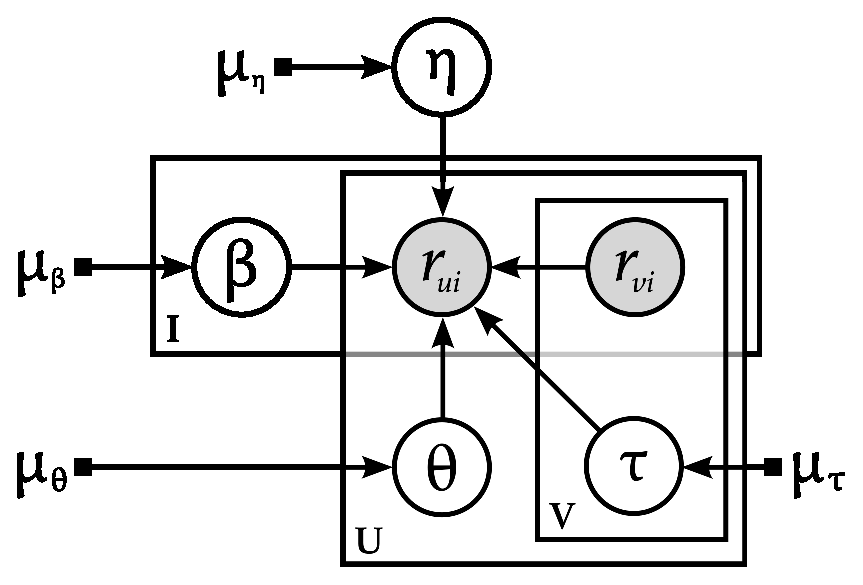
\includegraphics[width=0.69\linewidth]{../fig/graphicalmodel.eps}
    \vspace{-13px}
  \end{center}
  \caption{A conditional directed graphical model of social Poisson
    Factorization (SPF) to show considered dependencies.  For brevity, we refer to the set of priors $a$
    and $b$ as $\mu$; for example, $\mu_\theta = (a_\theta,
    b_\theta)$. These hyperparameters are fixed.}
  \label{fig:graphicalmodel}
\end{figure}

\mypar{Model specification.}  We formally describe SPF. The observed
data are user behavior and a social network.  The behavior data is a
sparse matrix $\mathbf{R}$, where $r_{ui}$ is the number of times user
$u$ clicked on item $i$. (Often this will be one or zero.) The social
network is represented by its neighbor sets; $N(u)$ is the set of
indices of other users connected to $u$.  Finally, the hidden
variables of SPF are per-user $K$-vectors of non-negative preferences
$\theta_u$, per-item $K$-vectors of non-negative attributes $\beta_i$,
and per-neighbor non-negative user influences $\tau_{uv}$. Loosely,
$\tau_{uv}$ represents how much user $u$ is influenced by the
clicks of her neighbor, user $v$.  (Note we must set the number of
components $K$.  Section~\ref{sec:eval} studies the effect of $K$ on
performance; usually we set it to 50 or 100.)

Conditional on the hidden variables and the social network, SPF is a
model of clicks $r_{ui}$.  Unlike many models in modern machine
learning, we specify the joint distribution of the entire matrix
$\mathbf{R}$ by the conditionals of each cell $r_{ui}$ given the
others,
\begin{equation}
  \label{eq:ratings}
  r_{ui} \, \vert \, r_{-u, i} \sim
  \mbox{Poisson}\left(\textstyle \theta_u^\top \beta_i + \sum_{v\in
      N(u)} \tau_{uv} r_{vi}\right),
\end{equation}
where $r_{-u, i}$ denotes the vector of clicks of the other users
of the $i$th item.\footnote{We are specifying an exponential family
  model conditionally.  This leads to a well-defined joint if and only
  if the natural parameters for each conditional are sums and products
  of the sufficient statistics of the corresponding conditionals of
  the conditioning set~\cite{Arnold1999}.  In our case, this is
  satisfied.} This equation captures the intuition behind the model,
that the conditional distribution of whether user $u$ clicks on item
$i$ is governed by two terms.  The first term, as we said above, is
the affinity between latent preferences $\theta_u$ and latent
attributes $\beta_i$; the second term bumps the parameter up when
trustworthy neighbors $v$ (i.e., those with high values of
$\tau_{uv}$) also clicked on the item.  Figure~\ref{fig:graphicalmodel}
shows the dependencies between the hidden and observed variables as
a conditional graphical model.

To complete the specification of the variables, we place gamma priors
on all of the hidden variables.  We chose the hyperparameters of the
gammas so that preferences, attributes, and influences are sparse.
(See Section~\ref{sec:eval} for details.)

\mypar{Forming recommendations with SPF.}  We have specified a
probabilistic model of hidden variables and observed clicks. Given
a $U \times I$ click matrix $\mathbf{R}$ and a $U \times U$ social
network $\mathbf{N}$, we analyze the data by estimating the posterior
distribution of the hidden preferences, attributes, and influences
$p(\theta_{1:U}, \beta_{1:I}, \tau_{1:U} \g \mathbf{R}, \mathbf{N})$.
This posterior places high probability on configurations of
preferences, attributes, and influence values that best describe the
observed clicks within the social network.

From this posterior, we can form predictions for each user and each of
their unclicked items.  For a user $u$ and an unclicked item $j$,
we compute
\begin{equation}
  \label{eq:recommendation}
  \E\left[r_{uj}\right] =
  \E\left[\theta_u\right]^\top \E\left[\beta_j\right] +
  \sum_{v \in N(u)} \E\left[\tau_{uv}\right] r_{vj},
\end{equation}
where all expectations are with respect to the posterior.  For each
user, we form recommendation lists by making predictions for the
user's set of unclicked items and then ranking the items by these
continuous-valued predictions.  This is how we can use SPF to form a
recommendation system.

\mypar{Learning the hidden variables with variational methods.}
Social PF enjoys the benefits of Poisson factorization and accounts
for the network of users.  However, using SPF requires computing
the posterior.  Conditioned on click data and a social
network, our goal is to compute the posterior user preferences, item
attributes, and latent influence values.

As for many Bayesian models, the exact posterior for SPF is not
tractable to compute; approximating the posterior is our central
statistical and computational problem.  We develop an efficient
approximate inference algorithm for SPF based on variational
methods~\cite{Bishop:2006,Jordan:1999}, a widely-used technique in
statistical machine learning for fitting complex Bayesian
models.\footnote{Source code available at \url{https://github.com/ajbc/spf}.}
With our algorithm, we can approximate posterior expectations with
very large click and network data (see Section~\ref{sec:eval}).

Variational inference approximates the posterior by solving an
optimization problem. We define a freely parameterized
distribution over the hidden variables, and then fit its parameters to
be close to the posterior distribution.  We measure ``closeness'' by
the Kullback-Leibler divergence, which is an assymetric measure of
distance between distributions.  Finally, we use the fitted
variational distribution as a proxy for the posterior, for example to
compute the expectations we need on the right-hand side of
Eq.~\ref{eq:recommendation}.

\begin{figure*}[t]
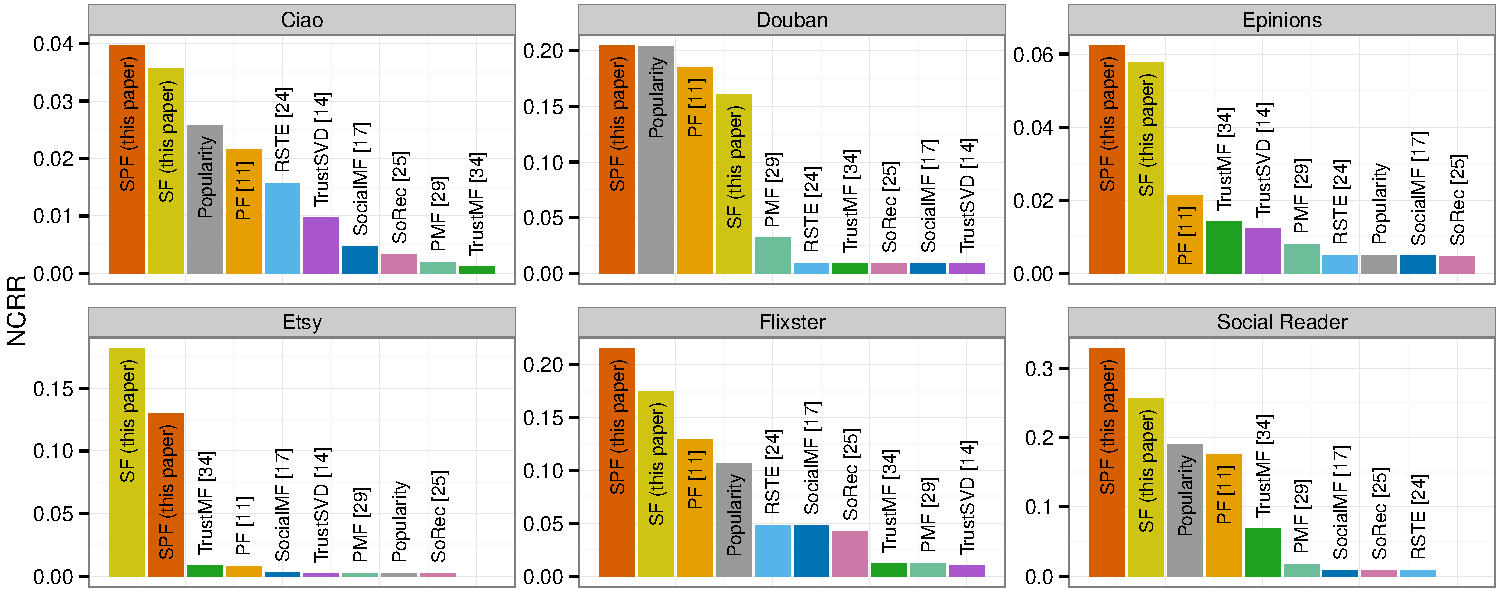
\includegraphics[width=\textwidth]{../fig/all.pdf}
\caption{Performance of various methods on all six datasets, measured
  as NCRR averaged over users with held-out data.  The Poisson-based
  factor models (PF and SPF) use $K=40$ on Ciao, $K=125$ on Epinions,
  $K=100$ on Etsy, and $K=50$ on Flixster, Douban, and Social Reader.
  Similar $K$ values are used for competing models, but some perform
  best with lower $K$, in which case those settings are used.  Models
  are sorted by performance.  RSTE was omitted on Etsy data due to
  long run time and TrustSVD was omitted on Social Reader data due to
  difficulty in finding appropriate parameter
  settings.  SPF outperforms all competing methods, except on Etsy,
  where our alternate model SF achieves top performance.}\label{fig:all}
\end{figure*}

We use the \textit{mean-field} variational family, where each latent
variable is independent and governed by its own varitional parameter.
The latent variables are the user preferences $\theta_u$, item
attributes $\beta_i$, and user influences $\tau_{uv}$.  The
variational family is
\begin{align}
  \label{eq:variational-distribution}
  q(\theta, \beta, \tau) = \prod_{u,k} q(\theta_{uk} \vert \lambda^\theta_{uk})
  \prod_{i,k} q(\beta_{ik} \vert \lambda^\beta_{ik})
  \prod_{u,v} q(\tau_{uv} \vert \lambda^\tau_{uv}).
\end{align}
This is a flexible family.  For example each cell of each user's
preference vector $\theta_{uk}$ is associated with its own variational
parameter $\lambda^\theta_{uk}$.  Thus, when fit to be close to the
model's posterior, the variational parameters can capture each user's
unique interests, each item's unique attributes, and each friend's
unique influence value.

With the family in place, variational inference solves the following
optimization problem,
\begin{equation}
  \label{eq:variational-problem}
  q^*(\theta, \beta, \tau) =
  \arg \min_{q} \mathrm{KL}\left(q(\theta, \beta, \tau) || p(\theta,
    \beta, \tau \g \mathbf{R}, \mathbf{N})\right).
\end{equation}
Note that the data---the clicks and the network---enter the
variational distribution through this optimization.  Finally, we use
the resulting variational parameters of $q^*(\cdot)$ as a proxy for
the exact posterior.  This lets us use SPF to perform recommendation.

In the appendix we describe the details of how we
solve the problem in Eq.~\ref{eq:variational-problem} to find a local
optimum of the KL divergence.  We use a form of alternating
minimization, iteratively minimizing the KL divergence with respect to
each of the variational parameters while holding the others fixed.
This leads to a scalable iterative algorithm, where each iteration
runs on the order of the number of non-zero entries of the matrix.
(In Section~\ref{sec:eval} we empirically compare the runtime of SPF
with competing methods.)  We now turn to an empirical study of SPF.


\section{Empirical Study}
\label{sec:eval}
In this section we study the performance of SPF.  We compared SPF to
five competing methods that involve a social network in
recommendation~\cite{guo2015trustsvd,Jamali:2010,Ma:2009,SoRec,Yang2013}
as well as two traditional factorization approaches~\cite{poisMF,PMF}.
Across six real-world datasets, our methods outperformed all of the
competing methods (Figure~\ref{fig:all}).  We also demonstrate how to
use SPF to explore the data, characterizing it in terms of latent
factors and social influence.  Finally, we assess sensitivity to the
number of latent factors and discuss how to set hyperparameters on the
prior distributions.

\subsection{Datasets, methods, and metrics}

\mypar{Datasets and preprocessing.} We studied six datasets.
Table~\ref{table:stats} summarizes their attributes.  The datasets
are:
\begin{itemize}
\setlength\itemsep{2px}
\item \textit{Ciao} (ciao.co.uk) is a consumer review website with an
  underlying social network.  Guo et al.~\cite{guo2014etaf} crawled
 DVD ratings and trust values for a small dataset of 7K users and 98K items.

\item \textit{Epinions} (epinions.com)
  is another consumer reviews website where users rate items
  and mark users as trustworthy.  Our data source was Massa and Avesani~\cite{Massa2007};
  the dataset consists of 39K users and 131K items.

\item \textit{Flixster} (flixster.com) is a social movie review
  website crawled by Jamali and Ester~\cite{Jamali:2010}.  We
  binarized ratings, thresholding at 3 or above, resulting in 132K users and 42K items.

\item \textit{Douban} (douban.com) is a Chinese social service where
  users record ratings for music, movies, and books; it was crawled by
  Ma et al.~\cite{hao:sr}.  It contains 129K users and 57K items.

\item \textit{Etsy} (etsy.com) is a marketplace for handmade and
  vintage items, as well as art and craft supplies.  Users may follow
  each other and mark items as favorites.  This data was provided
  directly by Etsy, and culled to users who have favorited at least 10 items and
  have at least 25\% of their items in common with their friends; we
  omitted any items with fewer than 5 favorites.  This is a large dataset of 40K users
  and 5.2M items.

\item \textit{Social Reader} is a dataset from a large media company
  that deployed a reader application on a popular online social
  network.  The data contains a friendship network and a table of
  article clicks.  We analyzed data from April 2-6, 2012, only
  including users who read at least 3 articles during that time.
  It contains 122K users and 6K items.

\end{itemize}

\begin{table*}[thb]
\centering
\begin{tabular}{c c c c c c c}
& \textbf{Ciao} & \textbf{Epinions} & \textbf{Flixster} & \textbf{Douban} & \textbf{Social Reader} & \textbf{Etsy} \\
\hline
\# of users & 7,375 & 39,307 & 131,542 & 129,097 & 121,950 & 39,862 \\
\# of items & 97,540 & 130,786 & 41,878 & 56,862 & 6,153 & 5,201,879 \\
\# user-item interactions & 270,427 & 639,775 & 6,740,332 & 16,207,151 & 489,735 & 18,650,632 \\
\% user-item interaction matrix & 0.038\% & 0.012\% & 0.122\% & 0.221\% & 0.065\% & 0.009\% \\
interaction type & 5-star & 5-star & binary (thresholded) & 5-star & binary (clicks) & binary (favoriting)\\
network type & directed & directed & undirected & undirected & undirected & directed \\
\# network connections & 56,267 & 176,337 & 488,869 & 1,323,828 & 100,175 & 4,761,437 \\
network edge density & 0.103\% & 0.011\% & 0.006\% & 0.016\% & 0.001\% & 0.300\% \\
\% shared & 25.0\% & 36.0\% & 62.3\% & 51.0\% & 50.1\% & 30.8\% \\
\end{tabular}
\caption{Attributes of each data source, post-curation.  User-item interactions are non-zero clicks, favorites, or ratings.  Percent
  shared is the average percentage of items users have in common with
  their friends.  Data sources were chosen for their diversity of attributes.}\label{table:stats}
\end{table*}
These datasets include both explicit ratings on a star scale and
binary data.  Content consumption is binary when the data is implicit
(a news article was viewed) or when the system only provides a binary
flag (favoriting).  With implicit data, non-Poisson models require us
to subsample 0's so as to differentiate between items; in these
instances, we randomly sampled negative examples such that each user
has the same number of positive and negative ratings.  Note that
Poisson-based models implicitly analyze the full matrix without
needing to pay the computational cost of analyzing the
zeros~\cite{poisMF}.

For each dataset, we preprocessed the network.  We removed network
connections where the users have no items in common.  Note this
advantages both SPF and comparison models (though SPF can learn the
relative influence of the neighbors).

Our studies divided the data into three groups: approximately 10\% of
1000 users' data are held-out for post-inference testing, 1\% of all users' data
are used to assess convergence of the inference algorithm (see
Appendix), and the rest is used to train.  One exception is Ciao,
where we used 10\% of all users' data to test.

\mypar{Competing methods.}  We compared SPF to five competing models
that involve a social network in recommendation: RSTE~\cite{Ma:2009},
TrustSVD~\cite{guo2015trustsvd}, SocialMF~\cite{Jamali:2010},
SoRec~\cite{SoRec}, and TrustMF~\cite{Yang2013}.\footnote{We used the LibRec library
  (librec.net) for all competing methods.} We also include probabilistic Gaussian matrix
factorization (PMF)~\cite{PMF}, because it is a widely used
recommendation method.  For each of these, we used the parameter
settings that achieved best performance according to the example fits
published on the LibRec website.

We can think of SPF having two parts: a Poisson factorization
component and a social component (see Eq.~\ref{eq:ratings}).
Thus we also compared SPF to each of these components in isolation,
Poisson factorization~\cite{poisMF} (PF) and \textit{social
  factorization} (SF).  SF is the influence model without the
factorization model.\footnote{Social factorization has a technical
  problem when none of a user's friends has clicked on an item; the
  resulting Poisson cannot have a rate of zero. Thus we add a small
  constant $\epsilon=10^{-10}$ to the rate in social factorization's
  model of clicks.}  We note that SF is a contribution of this paper.

Finally, we compare to two baselines, ordering items randomly and
ordering items by their universal popularity.

\mypar{Metrics.}  We evaluate these methods on a per-user basis.  For
each user, we predict clicks for both held-out and truly unclicked
items, and we rank these items according to their predictions.  We
denote the user-specific rank to be $\textrm{rank}_{ui}$ for item $i$
and user $u$.  A better model will place the held-out items higher in
the ranking (giving smaller $\textrm{rank}_{ui}$ values on held-out
items).  We now introduce the \textit{normalized cumulative reciprocal
  rank} (NCRR) metric to gauge this performance.

Reciprocal rank (RR) is an information retrieval measure; given a
query, it is the reciprocal of the rank at which the first relevant
document was retrieved.  (Larger numbers are better.)  Users ``query''
a recommender system similarly, except that each user only has one
query (e.g., ``what books should I read?'') and they care not just
about the first item that's relevant, but about finding as many
relevant items as possible.

Suppose user $u$ has held out items $\mathcal{D}_u$.\footnote{With
  binary data this is simply the full set of heldout items. When items
  have non-binary ratings, we threshold the set such to include only
  highly rated items ($4$ or $5$ in a $5$-star system).} We define the
cumulative reciprocal rank to be:
\[\textrm{CRR}_u = \sum_{i \in\mathcal{D}_u} \frac{1}{\mbox{rank}_{ui}}.\]
CRR can be interpreted as the ease of finding all held-out items, as
higher numbers indicate that the held-out items are higher in the
list.  For example, a CRR of 0.75 means that the second and fourth items
are in the held-out set, or are relevant to the user.

CRR behaves similarly to discounted cumulative gain (DCG), except it
places a higher priority on high-rank items by omitting the log
factor---it can be thought of as a harsher variant of DCG.  Like DCG,
it can be also be normalized.  The normalized cumulative reciprocal
rank (NCRR) is
\[\textrm{NCRR}_u = \frac{\textrm{CRR}_u}{\mbox{ideal}~\textrm{CRR}_u},\]
where the ideal variant in the denominator is the value of the metric
if the ranking was perfect.  To evaluate an entire model, we can
compute average NCRR over all users,
$\frac{1}{U}\sum_u \textrm{NCRR}_u$.  We will use this metric
throughout this section.


Performance measured by NCRR is consistent with performance measured
by NDCG, but NCRR is more interpretable---simple reciprocals are easier
to understand than the reciprocal of the log.

Note we omit root-mean-square error (RMSE) as a metric. Improvements
in RMSE often do not translate into accuracy improvements for ranked
lists~\cite{Amatriain:2012:WRU:2365952.2366042,topN,Loiacono:2014,Singh:2014},
especially with binary or implicit data.  Our end goal here is item
recommendation and not rating prediction---``which movie should I
watch next?'' is inherently a ranking problem---thus we treat the
predictions as means to an end.

\subsection{Performance and exploration}

We evaluate SPF by considering overall performance and performance as
a function of user degree.  We also show how to explore the data using the algorithm.

\mypar{Performance.} Figure~\ref{fig:all} shows the performance of SPF against the
competing methods: the previous methods that account for the
social network, social factorization (SF), Poisson factorization (PF),
and the popularity baseline.  (We do not illustrate the random baseline because it is
far below all of the other methods.)  SPF achieves top performance on
five of the datasets.  On the one remaining dataset, Etsy, the
social-only variant of our model (SF) performs best.

Notice the strong performance of ranking by popularity.  This
highlights the importance of social factorization.  It is only social
Poisson factorization that consistently outperforms this baseline.

\begin{figure}[ht]
\hspace{-10px}
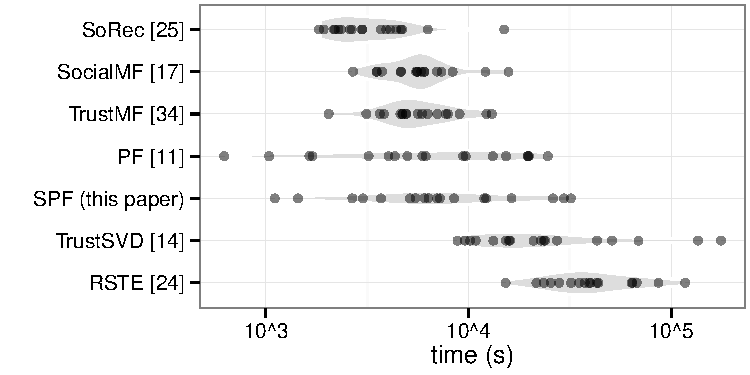
\includegraphics[width=\columnwidth]{../fig/runtimes.pdf}
\caption{Training and testing runtimes for multiple models on Ciao data, with the number of latent factors $K$ ranging from 1 to 500.  Each dot represents a full cycle of training and evaluating.  SPF performs with average runtime.}\label{fig:runtime}
\end{figure}

We measured runtime with the Ciao data set to get a sense for the
relative computational costs.  Figure~\ref{fig:runtime} shows the
runtime for all of the methods at various values of $K$.  The Poisson
models are average in terms of runtime.

Finally, using the Ciao and Epinions data, we break down the
performance of SPF, SF, and PF as a function of the degree of each
user; the results are shown in Figure~\ref{fig:degree}.\footnote{Smoothed with GAM. \url{http://www.inside-r.org/r-doc/mgcv/gam}}
All models perform better on high-degree users, presumably
because these are higher activity users as well. Overall, SPF performs
better than SF because of its advantage on the large number of
low-degree users.

\begin{figure}[ht]
\hspace{-10px}
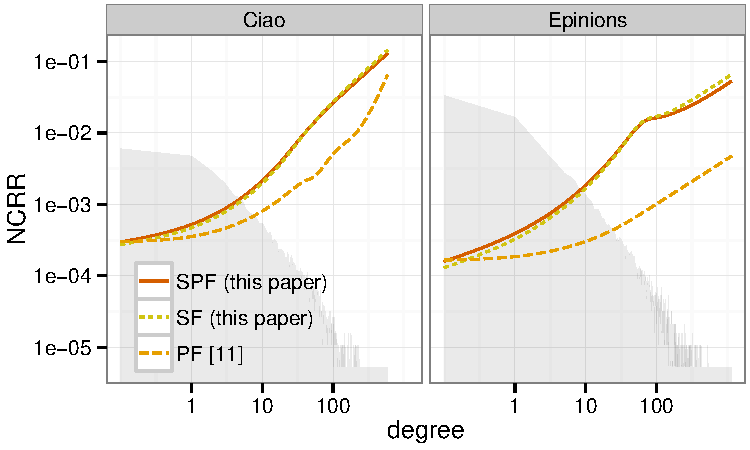
\includegraphics[width=\columnwidth]{../fig/ncrr_by_degree.pdf}
\caption{Performance on Ciao and Epinions broken down as a function of degree;
grey in background indicates density of users.  SPF and SF
perform similarly, with SPF doing slightly better on a large number of low-degree users
and SF doing better on a low number of high-degree users.}\label{fig:degree}
\end{figure}

\mypar{Interpretability.}  It is important to be able to explain the
origins of recommendations to users~\cite{Herlocker2000}.  Items
recommended with SPF have the advantage of interpretability.
In particular, we use auxiliary variables (see Appendix) to attribute each recommendation to friends or general preferences; we then use these attributions to explore data.

When items are recommended because
of social influence, the system may indicate a friend as the source of
the recommendation.
Similarly, when items are recommended because of general preferences, the system may indicate already clicked items that
exhibit that preference.
On the Etsy data, learned item factors included coherent groupings of items such as
mugs, sparkly nail polish, children's toys, handmade cards, and doll clothes.
Thus, SPF explains the recommended the handmade soap in Figure~\ref{fig:intuition}
as coming from general preferences and the others items as coming from social influence.
The social and preference signals will not always be cleanly separated; SPF attributes recommendations to sources probabilistically.

Figure~\ref{fig:preferences} shows how the proportion of social attribution (as opposed to
general preference attribution) changes as a function of user degree on Ciao and Epinions.  We observe that Epinions attributes a larger portion of behavior to social influence, controlled for user degree.  Similarly,
we can compute the contribution of users to their friends' behavior. Figure~\ref{fig:influence} shows social contribution as a function of indegree; here we see that Epinions users with higher indegree have lower social contribution than low-indegree users.

\begin{figure}[ht]
\hspace{-10px}
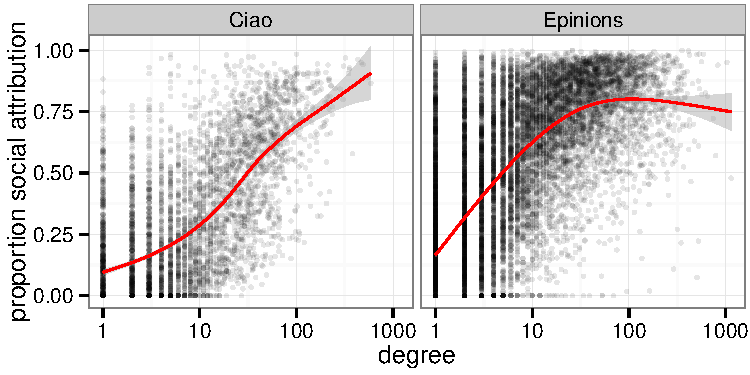
\includegraphics[width=\columnwidth]{../fig/preferences_by_degree.pdf}
\caption{The proportion of social attribution (vs. general preference attribution) as a function of user degree.
Attributions are calculated on all training data from Ciao and Epinions.  Epinions
attributes a larger portion of rating to social influence.}\label{fig:preferences}
\end{figure}

\begin{figure}[ht]
\hspace{-10px}
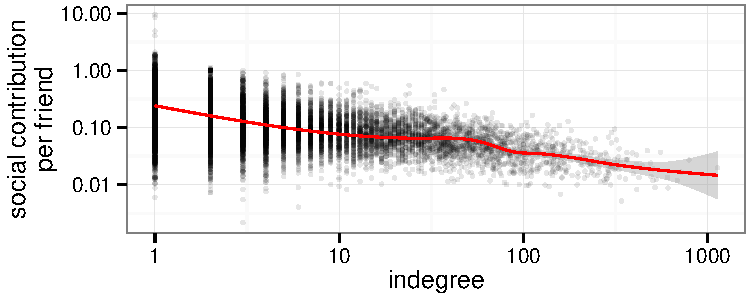
\includegraphics[width=\columnwidth]{../fig/influence_by_degree.pdf}
\caption{Contribution to friends' behavior as a function of indegree,
calculated on all Epinions training data.
Users with higher indegree have lower social contribution.
}\label{fig:influence}
\end{figure}


\subsection{Experimental details}

The details of our methods requires some decisions: we must choose the
number of latent factors $K$ and set the hyperparameters.

\mypar{Choosing the number of latent factors $K$.}  All factorization
models, including SPF, require the investigator to select of the
number of latent factors $K$ used to represent users and items.  We
evaluated the sensitivity to this choice for the Ciao dataset.  (We
chose this dataset because of its smaller size; ranking millions of
items for every user is computationally expensive for any model.)
Figure~\ref{fig:KsweepC} shows per-user average NCRR $K$ varies from 1
to 500; SPF performs best on the Ciao dataset with $K=40$, though is
less sensitive to this choice than some other methods (such as PF).

\begin{figure}[ht]
\hspace{-7px}
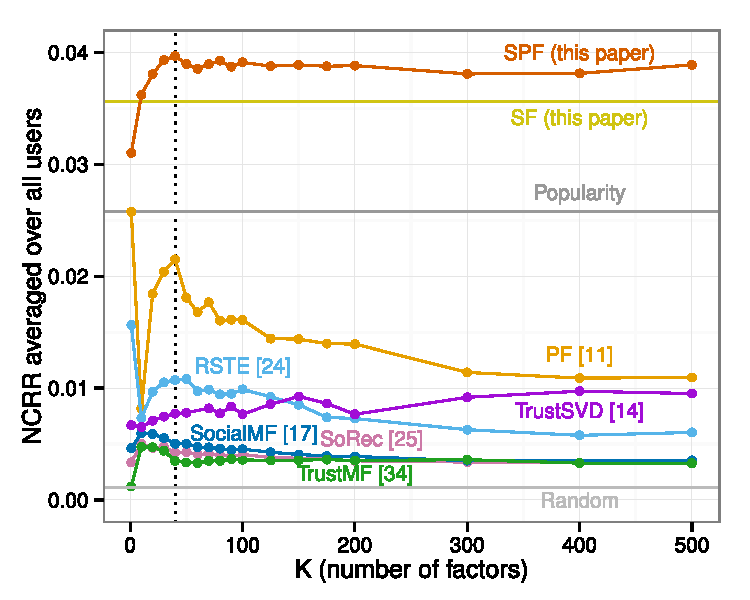
\includegraphics[width=\columnwidth]{../fig/k_sweep_Ciao.pdf}
\caption{Model performance on Ciao data (measured as NCRR averaged
  over all users) as a function of number of latent factors $K$.  The
  dotted vertical line at $K=40$ indicates the best performance for
  Poisson family models.}\label{fig:KsweepC}
\end{figure}

\mypar{Hyperparameters.}  We also must set the hyperparameters to the
gamma priors on the latent variables. The gamma is parameterized by a
shape and a rate.  We followed~\cite{poisMF} and set them to 0.3 for
the priors on latent preferences and attributes.  We set the
hyperparameters for the prior on user influences to $(2, 5)$ in order
to encourage the model to explore explanation by social influence.  In
a pilot study, we found that the model was not sensitive to these
settings.

\mypar{Does learning influence matter?} We can easily fix
each user-friend influence at 1, giving us local popularity among a
user's social connections.  We compared fitted influence against fixed
influence on both Ciao and Epinions and found that SPF with fitted
influence performs best on both datasets.

In the case of cold-start users, where we know the user's social
network but not their click counts on items, SPF will perform
equivalently to SF with fixed influence.  SPF in this
cold-start user scenario performs better than competing models.

\section{Discussion}
We presented social Poisson factorization, a Bayesian model that
incorporates a user's latent preferences for items with the latent
influences of her friends.  We demonstrated that social Poisson factorization improves recommendations
even with noisy online social signals.  Social Poisson
factorization has the following properties: (1) It discovers
the latent influence that exists between users in a social network,
allowing us to analyze the social dynamics. (2) It provides a source
of explainable serendipity (i.e., pleasant surprise due to novelty).
(3) It enjoys scalable algorithms that can be fit to large data sets.

We anticipate that social Poisson factorization will perform well on
platforms that allow for and encourage users to share content.
Examples include Etsy, Pinterest, Twitter, and Facebook.  We note that
our model does not account for time---when two connected
users both enjoy an item, one of them probably consumed it
first. Future work includes incorporating time, hierarchical
influence, and topical influence.

\section{Acknowledgments}
We thank Prem Gopalan, Jake Hofman, Chong Wang, Laurent Charlin, Rajesh Ranganath, and Alp Kucukelbir for their insights and discussions.  We thank Etsy, Diane Hu in particular, for sharing data.  We also thank LibRec's creator, Guibing Guo.
DMB is supported by NSF BIGDATA  NSF IIS-1247664, ONR N00014-11-1-0651, and DARPA FA8750-14-2-0009.
TER is supported by NSF CNS-1314603, by DTRA HDTRA1-10-1-0120, and by DAPRA under SMISC Program Agreement No. W911NF-12-C-0028.

\bibliographystyle{abbrv}
\begin{thebibliography}{10}

\bibitem{Amatriain:2012:WRU:2365952.2366042}
X.~Amatriain, P.~Castells, A.~de~Vries, and C.~Posse.
\newblock Workshop on recommendation utility evaluation: Beyond {RMSE}.
\newblock In {\em RecSys}, pages 351--352, 2012.

\bibitem{Andersen2008}
R.~Andersen, C.~Borgs, J.~Chayes, U.~Feige, A.~Flaxman, A.~Kalai, V.~Mirrokni,
  and M.~Tennenholtz.
\newblock Trust-based recommendation systems: an axiomatic approach.
\newblock In {\em WWW}, pages 199--208, 2008.

\bibitem{Arnold1999}
B.~C. Arnold, E.~Castillo, and J.~M. Sarabia.
\newblock {\em Conditional specification of statistical models}.
\newblock Springer, 1999.

\bibitem{Bishop:2006}
C.~Bishop.
\newblock {\em Pattern Recognition and Machine Learning}.
\newblock Springer New York, 2006.

\bibitem{CannyGaP}
J.~Canny.
\newblock {GaP}: a factor model for discrete data.
\newblock In {\em SIGIR}, pages 122--129, 2004.

\bibitem{Crandall2008}
D.~Crandall, D.~Cosley, D.~Huttenlocher, J.~Kleinberg, and S.~Suri.
\newblock Feedback effects between similarity and social influence in online
  communities.
\newblock In {\em KDD}, pages 160--168, 2008.

\bibitem{topN}
P.~Cremonesi, Y.~Koren, and R.~Turrin.
\newblock Performance of recommender algorithms on top-n recommendation tasks.
\newblock In {\em RecSys}, pages 39--46, 2010.

\bibitem{Du:2013}
N.~Du, L.~Song, H.~Woo, and H.~Zha.
\newblock Uncover topic-sensitive information diffusion networks.
\newblock In {\em {AISTATS}}, pages 229--237, 2013.

\bibitem{Fazeli:2014}
S.~Fazeli, B.~Loni, A.~Bellogin, H.~Drachsler, and P.~Sloep.
\newblock Implicit vs. explicit trust in social matrix factorization.
\newblock In {\em RecSys}, pages 317--320, 2014.

\bibitem{FilmTrust}
J.~Golbeck and J.~Hendler.
\newblock Film{T}rust: {M}ovie recommendations using trust in web-based social
  networks.
\newblock {\em TOIT}, 6(4):497--529, Jan. 2006.

\bibitem{poisMF}
P.~Gopalan, J.~M. Hofman, and D.~M. Blei.
\newblock Scalable recommendation with hierarchical {P}oisson factorization.
\newblock In {\em UAI}, pages 326--335, 2015.

\bibitem{Guille:2013}
A.~Guille, H.~Hacid, C.~Favre, and D.~A. Zighed.
\newblock Information diffusion in online social networks: A survey.
\newblock {\em SIGMOD Record}, 42(2):17--28, July 2013.

\bibitem{guo2014etaf}
G.~Guo, J.~Zhang, D.~Thalmann, and N.~Yorke-Smith.
\newblock Etaf: An extended trust antecedents framework for trust prediction.
\newblock In {\em ASONAM}, pages 540--547, 2014.

\bibitem{guo2015trustsvd}
G.~Guo, J.~Zhang, and N.~Yorke-Smith.
\newblock Trust{SVD}: Collaborative filtering with both the explicit and
  implicit influence of user trust and of item ratings.
\newblock {\em AAAI}, pages 123--129, 2015.

\bibitem{Herlocker2000}
J.~L. Herlocker, J.~A. Konstan, and J.~Riedl.
\newblock Explaining collaborative filtering recommendations.
\newblock In {\em CSCW}, pages 241--250, 2000.

\bibitem{Hoffman:2013}
M.~Hoffman, D.~Blei, C.~Wang, and J.~Paisley.
\newblock Stochastic variational inference.
\newblock {\em Journal of Machine Learning Research}, 14(1303--1347), 2013.

\bibitem{Jamali:2010}
M.~Jamali and M.~Ester.
\newblock A matrix factorization technique with trust propagation for
  recommendation in social networks.
\newblock In {\em RecSys}, pages 135--142, 2010.

\bibitem{Johnstone1957}
J.~Johnstone and E.~Katz.
\newblock Youth and popular music: A study in the sociology of taste.
\newblock {\em Journal of Sociology}, 62(6):563--568, May 1957.

\bibitem{Jordan:1999}
M.~I. Jordan, Z.~Ghahramani, T.~S. Jaakkola, and L.~K. Saul.
\newblock An introduction to variational methods for graphical models.
\newblock {\em Machine Learning}, 37(2):183--233, Nov. 1999.

\bibitem{Koren09}
Y.~Koren, R.~Bell, and C.~Volinsky.
\newblock Matrix factorization techniques for recommender systems.
\newblock {\em IEEE Computer}, 42:30--37, 2009.

\bibitem{Lee00}
D.~D. Lee and H.~S. Seung.
\newblock Algorithms for non-negative matrix factorization.
\newblock In {\em NIPS}, pages 556--562, 2000.

\bibitem{Leskovec:2006}
J.~Leskovec, A.~Singh, and J.~Kleinberg.
\newblock Patterns of influence in a recommendation network.
\newblock In {\em PAKDD}, pages 380--389, 2006.

\bibitem{Loiacono:2014}
D.~Loiacono, A.~Lommatzsch, and R.~Turrin.
\newblock An analysis of the 2014 recsys challenge.
\newblock In {\em RecSysChallenge}, page~1, 2014.

\bibitem{Ma:2009}
H.~Ma, I.~King, and M.~R. Lyu.
\newblock Learning to recommend with social trust ensemble.
\newblock In {\em SIGIR}, pages 203--210, 2009.

\bibitem{SoRec}
H.~Ma, H.~Yang, M.~R. Lyu, and I.~King.
\newblock So{R}ec: Social recommendation using probabilistic matrix
  factorization.
\newblock In {\em CIKM}, pages 931--940, 2008.

\bibitem{hao:sr}
H.~Ma, D.~Zhou, C.~Liu, M.~R. Lyu, and I.~King.
\newblock Recommender systems with social regularization.
\newblock In {\em WSDM}, pages 287--296, 2011.

\bibitem{Massa2007}
P.~Massa and P.~Avesani.
\newblock Trust-aware recommender systems.
\newblock In {\em RecSys}, pages 17--24, 2007.

\bibitem{CTRrec2012}
S.~Purushotham, Y.~Liu, and C.-C.~J. Kuo.
\newblock Collaborative topic regression with social matrix factorization for
  recommendation systems.
\newblock {\em CoRR}, abs/1206.4684, 2012.

\bibitem{PMF}
R.~Salakhutdinov and A.~Mnih.
\newblock Probabilistic matrix factorization.
\newblock In {\em NIPS}, pages 1257--1264, 2007.

\bibitem{WisdomOfCrowd}
S.~Shang, P.~Hui, S.~R. Kulkarni, and P.~W. Cuff.
\newblock Wisdom of the crowd: Incorporating social influence in recommendation
  models.
\newblock In {\em ICPADS}, pages 835--840, 2011.

\bibitem{Singh:2014}
P.~Singh, G.~Singh, and A.~Bhardwaj.
\newblock Ranking approach to recsys challenge.
\newblock In {\em RecSysChallenge}, page~19, 2014.

\bibitem{CFsurvey}
X.~Su and T.~M. Khoshgoftaar.
\newblock A survey of collaborative filtering techniques.
\newblock {\em Advances in Artificial Intelligence}, page~4, Jan. 2009.

\bibitem{Volz2006}
I.~P. Volz.
\newblock The impact of online music services on the demand for stars in the
  music industry.
\newblock In {\em WWW}, pages 659--667, 2006.

\bibitem{Yang2013}
B.~Yang, Y.~Lei, D.~Liu, and J.~Liu.
\newblock Social collaborative filtering by trust.
\newblock In {\em IJCAI}, pages 2747--2753, 2013.

\bibitem{Ye:2012}
M.~Ye, X.~Liu, and W.-C. Lee.
\newblock Exploring social influence for recommendation: A generative model
  approach.
\newblock In {\em SIGIR}, pages 671--680, 2012.

\bibitem{SBPR}
T.~Zhao, J.~McAuley, and I.~King.
\newblock Leveraging social connections to improve personalized ranking for
  collaborative filtering.
\newblock In {\em CIKM}, pages 261--270, 2014.

\end{thebibliography}

\normalsize

\appendix
\label{app:inference}
In this appendix, we describe the details of the variational inference
algorithm for SPF.  This algorithm fits the parameters of the
variational distribution in Eq.~\ref{eq:variational-distribution}
so that it is close in KL divergence to the posterior.  We use
coordinate ascent, iteratively updating each parameter while holding
the others fixed.  This goes uphill in the variational objective and
converges to a local optimum~\cite{Bishop:2006}.

To obtain simple updates, we first construct auxiliary latent
variables $z$.  These variables, when marginalized out, leave the
original model intact.  Recall the additive property of the Poisson
distribution.  Specifically, if $r \sim \mbox{Poisson}(a+b)$ then
$r = z_1 + z_2$, where $z_1 \sim \mbox{Poisson}(a)$ and
$z_2 \sim \mbox{Poisson}(b)$.  We apply this decomposition to the
conditional click count distribution in Eq.~\ref{eq:ratings}.  We
define Poisson variables for each term in the click count:
\begin{equation*}
  z^M_{uik} \sim \mbox{Poisson}(\theta_{uk}\beta_{ik}) \quad
  z^S_{uiv} \sim \mbox{Poisson}\left(\tau_{uv} r_{vi}\right).
\end{equation*}
The $M$ and $S$ superscripts indicate the contributions from matrix
factorization (general preferences) and social factorization
(influence), respectively.  Given these variables, the click count is
deterministic,
\begin{equation*}
  r_{ui} \, \vert \, r_{-u,i} = \textstyle \sum_{k=1}^K z^M_{uik} + \sum_{v=1}^V
  z^S_{uiv},
\end{equation*}
where $V=\vert N(u) \vert$ and the index $v$ selects a friend of $u$
(as opposed to selecting from the set of all users).

Coordinate-ascent variational inference is derived from the complete
conditionals, i.e., the conditional distributions of each variable
given the other variables and observations.  These conditionals define
both the form of each variational factor and their updates.  For the
Gamma variables---the user preferences, item attributes, and user
influence---the conditionals are {\small
\begin{eqnarray}
  \hspace{-15px}\textstyle \theta_{uk} ~\vert~ \beta, \tau, z, \mathbf{R}, \mathbf{N}&\hspace{-7px}\sim&\hspace{-7px}
  	\textrm{Gam}\left(a_\theta + \sum_{i} z_{uik}^M ,~
  	b_\theta+ \sum_{i}\beta_{ik} \right) \label{eq:thetaCC}\\
  \hspace{-15px}\textstyle \beta_{ik} ~\vert~ \theta, \tau, z, \mathbf{R}, \mathbf{N}&\hspace{-7px}\sim&\hspace{-7px}
  	\textrm{Gam}\left(a_\beta + \sum_u z_{uik}^M ,~
  	b_\beta+ \sum_u\theta_{uk} \right) \label{eq:betaCC} \\
  \hspace{-15px}\textstyle \tau_{uv} ~\vert~ \theta, \beta, z, \mathbf{R}, \mathbf{N}&\hspace{-7px}\sim&\hspace{-7px}
  	\textrm{Gam}\left(a_\tau + \sum_{i} z_{uiv}^S,~
	b_\tau+ \sum_{i} r_{vi} \right).
	\label{eq:tauCC}
\end{eqnarray}
}The complete conditional for the auxiliary variables is \\
\noindent$z_{ui} ~\vert~ \theta, \beta, \tau, \mathbf{R}, \mathbf{N} \sim
\mbox{Mult}\left(r_{ui}, \phi_{ui}\right)$ where
\begin{equation}
\phi_{ui} \propto \bigg\langle \theta_{u1}\beta_{i1},~\cdots, ~\theta_{uK}\beta_{iK},
  \tau_{u1}r_{1i},~\cdots,~ \tau_{uV}r_{Vi}
      \bigg\rangle.
\label{eq:phi}
\end{equation}
(Intuitively, these variables allocate the data to one of the factors
or one of the friends.)  Each variational factor is set to the same
family as its corresponding complete conditional.

Given these conditionals, the algorithm sets each parameter to the
expected conditional parameter under the variational distribution.
(Thanks to the mean field assumption, this expectation will not
involve the parameter being updated.)  Note that under a gamma
distribution, $\E[\lambda] = \lambda_a / \lambda_b,$ where $\lambda_a$
and $\lambda_b$ are shape and rate parameters.  For the auxiliary
variables, the expectation of the indicator is the probability,
$\E[z_{ui}] = r_{ui} * \phi_{ui}$.

Algorithm~\ref{alg:SPF} shows our variational inference algorithm.  It
is $O(N(K+V))$ per iteration, where $N$ is the number of recorded
user-item interactions (click counts, ratings, etc.). $K$ is the
number of latent factors, and $V$ is the maximum user degree.  (Note
that both $K$ and $V$ are usually small relative to $N$.)  We can modify
the algorithm to sample users and update the variables
stochastically~\cite{Hoffman:2013}; this approach scales to much
larger datasets than competing methods.

\alglanguage{pseudocode}
\begin{algorithm}[h]
\small
\caption{Mean field variational inference SPF}
\label{alg:SPF}
\begin{algorithmic}[1]
\State initialize $\E[\theta], \E[\beta]$ randomly
\For {each user $u$}
	\For {each friend $v\in N(u)$}
		\State $\lambda^{\tau,b}_{u,v} =  \mbox{prior~} b_{\tau} + \sum_i r_{vi}$
		\Comment{\mbox{see Eq.~\ref{eq:tauCC}}}
	\EndFor
\EndFor
\While {$\Delta\log\mathcal{L} > \delta$}
 \Comment{\mbox{check for model convergence}}
	\State {init.~global $\lambda^{\beta,a}$ to prior $a_\beta$ for all items and all factors}
	\For {each user $u$}
		\While{$\Delta\mathbf[\theta_{u}] + \Delta\mathbf[\tau_{u}] > \delta'$}
		\Comment{\mbox{user convergence}}
			\State init.~local $\lambda^{\beta,a}$ to 0 for all items and factors
			\State init.~preferences $\lambda^{\theta,a}_{u}$ to prior $a_\theta$ for all factors
			\State $\lambda^{\theta,b}_{u} =  \mbox{prior~} b_{\theta} + \sum_i \E[\beta_i]$
			\Comment{\mbox{see Eq.~\ref{eq:thetaCC}}}
			\State init. influence $\lambda^{\tau,a}_{user}$ to prior $a_\tau$ for all friends
			\For {each (item $i$, click count $r$) $\in clicks_{u}$}
				\State set $\phi_{ui}$ from $\E[\theta_{u}]$, $\E[\beta_{i}]$,
				$\E[\tau_{u}]$, and $r_i$ (Eq.~\ref{eq:phi})
				\State $\E[z_{ui}] = r~*~\phi_{ui} $
				\State update $\lambda^{\theta,a}_{u} \pluseq \E[z_{ui}^M]$  \Comment{\mbox{see Eq.~\ref{eq:thetaCC}}}
				\State update $\lambda^{\tau,a}_{u} \pluseq \E[z_{ui}^S]$  \Comment{\mbox{see Eq.~\ref{eq:tauCC}}}
				\State update local $\lambda^{\beta,a}_{i} \pluseq \E[z_{ui}^M]$  \Comment{\mbox{see Eq.~\ref{eq:betaCC}}}
			\EndFor

			\State $\E[\theta_{u}] = \lambda^{\theta,a}_{u} / \lambda^{\theta,b}_{u}$
			\State $\E[\tau_{u}] = \lambda^{\tau,a}_{u} / \lambda^{\tau,b}_{u}$

		\EndWhile

		\State global $\lambda^{\beta,a} \pluseq $ local $\lambda^{\beta,a}$
	\EndFor
	\State $\lambda^{\beta,b} = \mbox{prior~} b_{\beta} + \sum_u \E[\theta_u]$\Comment{\mbox{see Eq.~\ref{eq:betaCC}}}
	\State $\E[\beta] = \lambda^{\beta,a} / \lambda^{\beta,b}$
\EndWhile
\end{algorithmic}
\end{algorithm}

To assess convergence, we use the change in the average click log likelihood of a validation set.

\balancecolumns

\end{document}

